\documentclass{beamer}
\beamertemplatenavigationsymbolsempty
\usepackage{tikz}
\begin{document}


\begin{frame}{Where were we? Colouring graphs}
\begin{itemize}
    \item Chromatic number $\chi(G)$: colour vertices with fewest colours
    \item Chromatic index $\chi^\prime(G)$: colour edges with fewest colours
    \item Chromatic polynomial $P_G(k)$: number of ways to colour vertices with $k$ colours
\end{itemize}


\begin{columns}
   \begin{column}{.6\textwidth}
 \begin{block}{Some graphs: colour vertex by vertex}
$$P_G(k)=k(k-1)^4(k-2)^2$$
\end{block}
\begin{block}{In general: need case-by-case}
Examples we looked at: $C_4, C_5$.
\end{block}
\end{column}
        
      \begin{column}{.4\textwidth}
        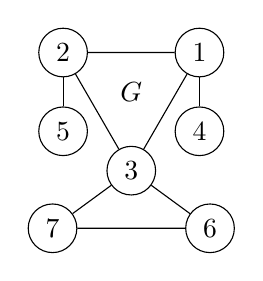
\begin{tikzpicture}
 \draw node at (0,0) {$G$};
          \begin{scope}[every node/.style={circle, draw}]
          \node (1) at (30:1) {$1$};
          \node (2) at (150:1) {$2$};
          \node (3) at (-90:1) {$3$};
          \node (4) at (-30:1) {$4$};
          \node (5) at (210:1) {$5$};
          \node (6) at (-60:2) {$6$};
          \node (7) at (-120:2) {$7$};
          \draw (6)--(3)--(1)--(2)--(3)--(7)--(6);
          \draw (1)--(4);
          \draw (2)--(5);
        
          \end{scope}
          \end{tikzpicture}
        \end{column}  
    \end{columns}
\begin{block}{Today: prove $P_G(k)$ is a polynomial}
\end{block}
  \end{frame}
  
\begin{frame}{Review: Chromatic polynomial of $C_4$ and a Lemma}  
\begin{lemma}Let $x$ and $y$ be two non-adjacent vertices in $G$.  Then 
$$P_G(k)=P_{G_{+xy}}(k)+P_{G_{x=y}}(k)$$
\end{lemma}

  \begin{columns}
     \begin{column}{.5\textwidth}
\begin{block}{1 and 3 have different colours}

  \centering
  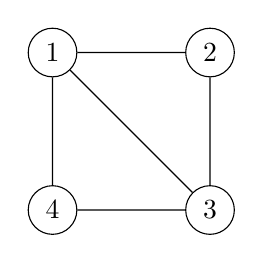
\begin{tikzpicture}[scale=2]
\begin{scope}[every node/.style={circle, draw}]
\node (1) at (0,1) {$1$};
\node (2) at (1,1) {$2$};
\node (3) at (1,0) {$3$};
\node (4) at (0,0) {$4$};
\draw (1)--(2)--(3)--(4)--(1)--(3);
\end{scope}
\end{tikzpicture}
$k(k-1)(k-2)^2$
\end{block}
     \end{column}
 \begin{column}{.5\textwidth}
\begin{block}{1 and 3 have the same colour}

  \centering
  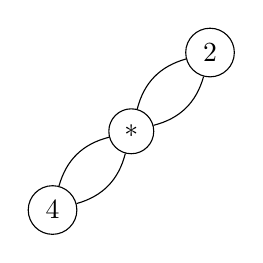
\begin{tikzpicture}[scale=2]
\begin{scope}[every node/.style={circle, draw}]
\node (1) at (.5,.5) {$*$};
\node (2) at (1,1) {$2$};
\node (4) at (0,0) {$4$};
\draw (2) to[bend right] (1);
\draw (1) to[bend right] (4);
\draw (4) to[bend right] (1);
\draw (1) to[bend right] (2);
\end{scope}
  \end{tikzpicture}
  
$k(k-1)^2$
\end{block}
     \end{column}
  \end{columns}
$$P_{C_4}(k)=k(k-1)(k-2)^2+k(k-1)^2=k(k-1)(k^2-3k+3)$$  
  \end{frame}
\begin{frame}{Deletion-Contraction: restructuring the lemma}
The lemma as stated is useful for calculating, but awkward for induction:
\begin{itemize}
    \item $G_{+xy}$ has an extra edge; "bigger"
    \item $G_{x=y}$ has fewer vertices: "smaller"
\end{itemize}
Rewrite so $H\cong G_{+xy}$ is the "starting" graph.
\begin{lemma}[Deletion-Contraction]
Let $H$ be a graph, and let $e$ be an edge in $H$.  Then
$$P_H(k)=P_{H\setminus e}(k)-P_{H/e}(k)$$
\end{lemma}  
The edge $e$ is between $xy$
$$H=G+xy,\qquad H\setminus e=G,\qquad H/e=G_{x=y}$$

\end{frame}  

\begin{frame}{Brief Advertisements}
\makebox[\linewidth]{\includegraphics[width=\paperwidth]{Pictures/CareerServices.jpg}}
\end{frame}


\begin{frame}{Chromatic polynomial is a polynomial}
\begin{theorem}
Let $G$ be a simple graph. Then $P_G(k)$ is a polynomial in $k$.  

Moreover, if $G$ has $n$ vertices and $m$ edges, then 
$$P_G(k)=k^n-mk^{n-1}+\text{lower order terms}$$
\end{theorem}

\begin{block}{Proof idea:}
Induct on the number of edges using deletion-contraction.
\end{block}
\begin{block}{Base case: $m=0$}
If $G$ has no edges and $n$ vertices, then $G=E_n$ empty graph.
$P_{E_n}=k^n$ is a polynomial of the right form.
\end{block}

\end{frame}
\begin{frame}{Inductive step}
Assume that $G$ has $m>0$ edges and $n$ vertices, and that for any graph $H$ with $\ell<m$ edges and $p$ vertices, we have $P_H(k)=k^p-\ell k^{p-1}+\cdots$.

\begin{block}{Let $e\in G$ be any edge:}
\begin{itemize}
    \item $G\setminus e$ has $n$ vertices and $m-1$ edges
    \item $G/e$ has $n-1$ vertices and \emph{at most} $m-1$ edges
\end{itemize}
So by the inductive hypothesis, theorem holds for $G\setminus e$ and $G/e$
\end{block}
\begin{block}{So applying Deletion-Contraction:}\begin{align*}
    P_G(k) &= P_{G\setminus e}(k)-P_{G/e}(k) \\
    &= \left(k^n-(m-1)k^{n-1} +\cdots\right) -\left(k^{n-1}-\cdots\right) \\
    &= k^n-mk^{n-1}+\cdots
\end{align*}
Which is what we needed to show. \quad$\square$
\end{block}

\end{frame}
\begin{frame}{Odds and Ends}
  \begin{block}{Deletion-Contraction as an algorithm}
    \begin{itemize}
    \item Can always find $P_G(x)$ by iterating deletion-contraction
    \item In practise, often faster to add edges
      \end{itemize}
  \end{block}

  \begin{block}{Information in $P_G(k)$}
    \begin{itemize}
    \item Number of vertices is the degree
    \item Number of edges is negative the coefficient of next highest term
      \item $\chi(G)$ is the lowest $k$ with $P_G(k)\neq 0$.
\end{itemize}

    \end{block}

    



\end{frame}


\end{document}
